\documentclass[12pt]{jarticle}
\usepackage{a4wide}
\usepackage{amsmath}%数学記号
\usepackage{amssymb}%数学記号
\usepackage{epsfig}%図
\usepackage{latexsym}
\usepackage{supertabular}
\usepackage{graphicx}
\usepackage{color}
\usepackage{ascmac}
\usepackage{multicol}
\usepackage{ascmac}
\usepackage{systeme}
\usepackage{amsmath,cases}
\usepackage{float}
\usepackage{here}
\pagestyle{plain}

\newtheorem{theorem}{定理}[section]
\newtheorem{lemma}[theorem]{補題}
\newtheorem{proposition}[theorem]{命題}
\newtheorem{conjecture}[theorem]{予想}
\newtheorem{corollary}[theorem]{系}
\newtheorem{definition}[theorem]{定義}
\newtheorem{example}[theorem]{例}
\newtheorem{exercise}[theorem]{例題}
\newtheorem{problem}[theorem]{問}
\newtheorem{algorithm}[theorem]{アルゴリズム}
\newtheorem{remark}[theorem]{注意}

\def\qed{{\hfill$\square$}}
\def\proof{{\vspace{-0.3cm}f 証明: \,}}
\def\solution{{\vspace{-0.3cm}f 解: \,}}
\def\N{{\Bbb N}}
\def\Z{{\Bbb Z}}
\def\Q{{\Bbb Q}}
\def\R{{\Bbb R}}
\def\C{{\Bbb C}}
\def\F{{\Bbb F}}
\def\D{{\mathcal D}}
\def\mod{{\mathrm{mod\,\,}}}
\def\GL{{\mathrm{GL}}}
\def\GF{{\mathrm{GF}}}
\def\H{{\mathcal{H}}}

\setlength{\textwidth}{170mm}
\setlength{\textheight}{240mm}
\setlength{\oddsidemargin}{-5mm}
\setlength{\evensidemargin}{-5mm}
\setlength{\topmargin}{-10mm}
\setlength{\headheight}{0mm}
\setlength{\headsep}{10mm}

\title{項目反応理論}
\begin{document}
\maketitle
\setcounter{section}{4}
\setcounter{subsection}{2}
\subsection{ベイズ推定法}
本節では$3.4$節で導入したベイズ推定法を項目母数の推定に利用する方法を論じていく。周辺推定法では、被験者が全員正答、全員誤答した項目の項目母数は推定することができなかったが、ベイズ推定法なら可能である。それ自体が問題になるわけではないが、事前分布が適切である場合にはベイズ推定法は実用的には便利な方法である。ここでベイズの公式を再掲したものが以下である。
\begin{align}
  \label{00}
  \displaystyle f(A|B) = \frac{f(A)f(B|A)}{f(B)}\tag{4.29}
\end{align}
ここでは、反応パタンが与えられたときの母数に事後分布を求めるので、$A$は$\boldsymbol{\theta,a,b,c}$に相当し、$B$は、$\boldsymbol{U}$に相当する。
\subsubsection{同時尤度による方法}
はじめに、$f(A)$に相当する事前分布を導く。ここでは、全ての母数は独立しており、ある確率分布$g(\cdot)$に従ってランダムに分布していることを仮定している。独立の仮定の下で、複数の母数の事前分布はその総積で
\begin{align}
  \label{01}
  \displaystyle
  g(\boldsymbol{\theta,a,b,c}) = \prod_{i = 1}^{N}g(\theta_i) \prod_{j = 1}^{n} g(a_i)g(b_i)g(c_i)  \tag{4.30}
\end{align}
と表現される。これを同時事前分布という。
被験者母数の事前分布$g(\theta_i)$には正規分布が識別力の事前分布$g(a_j)$には、対数正規分布が、困難度の事前分布$g(b_j)$には正規分布が、当て推量の事前分布$g(c_j)$にはベータ分布が仮定されることが多い。
式$(4.9)$の$L(\boldsymbol{U}|\boldsymbol{\theta,a,b,c}) = f(\boldsymbol{U}|\boldsymbol{\theta,a,b,c})$と式$(4.29)$ $\displaystyle f(A|B) = \frac{f(A)f(B|A)}{f(B)}$を用いると、
\begin{align}
  \label{02}
  \displaystyle
  f(\boldsymbol{L}|\boldsymbol{\theta,a,b,c}) = \frac{g(\boldsymbol{\theta,a,b,c})L(\boldsymbol{U}|\boldsymbol{\theta,a,b,c})}{f(\boldsymbol{U})} \tag{4.31}
\end{align}
のように表現することができる。この式を$\boldsymbol{\theta,a,b,c}$に関して最大化し、ベイズ推定値を得る。実際には積の連なりであることが多いので対数変換を行って母数で偏微分し$0$と置き連立方程式を解く。母数で偏微分した時点で、分母の$f(\boldsymbol{U})$は$0$になるので、分子の最大化を考えればよい。
\subsubsection{周辺尤度による方法}
ここでは、周辺化によって被験者母数を消去して母数の数を減らす方法を紹介する。まず、周辺化により被験者母数を消去すると、項目母数の同時事後分布は
\begin{align}
  \label{03}
  \displaystyle
  f(\boldsymbol{a,b,c}|\boldsymbol{U}) = \int f(\boldsymbol{\theta,a,b,c}|\boldsymbol{U}) d\boldsymbol{\theta} \tag{4.32}
\end{align}と表現される。(理由は以下で説明する)
\begin{itembox}[l]{連続型確率変数}
  連続型確率変数$\boldsymbol{X,Y}$では、それぞれの実現値$x,y$と確率密度$f(x),f(y)$に関して以下が成り立つ.
  \begin{align}
    \label{04}
    \displaystyle
    \int f(x|y)dx = 1
    \tag{4.33}
  \end{align}から確率変数の連なりに置き換えて
  \begin{align}
    \label{05}
    \displaystyle
    \int f(x,y|z)dy = f(x|z)
    \tag{4.34}
  \end{align}
\end{itembox}
式($4.32$)を$\boldsymbol{a,b,c}$に関して最大化し、ベイズ推定値を得る。
\subsubsection{被験者母数の事前分布}
上記に示したように、被験者母数の事前分布には正規分布が仮定されることが多い。正規分布の母数は平均$\mu_\theta$と分散${\sigma}^2 _\theta$である。
\subsubsection{困難度の事前分布}
困難度の事前分布にも正規分布が仮定されることが多い。被験者母数の事前分布を$\mu_\theta = 0,{\sigma}^2 _\theta = 1$で設定する場合にはそれより広い範囲をカバーする事前分布を仮定する必要がある。あるソフトウェアでは$\mu_\theta = 0,{\sigma}^2 _\theta = 4$で設定されているものもある。
\subsubsection{識別力の事前分布}
識別力は原理的には、負の値もとり得る。そこで、識別力の事前分布には正の範囲で定義される対数正規分布が仮定されることが多い。
\begin{center}
\begin{figure}[H]
  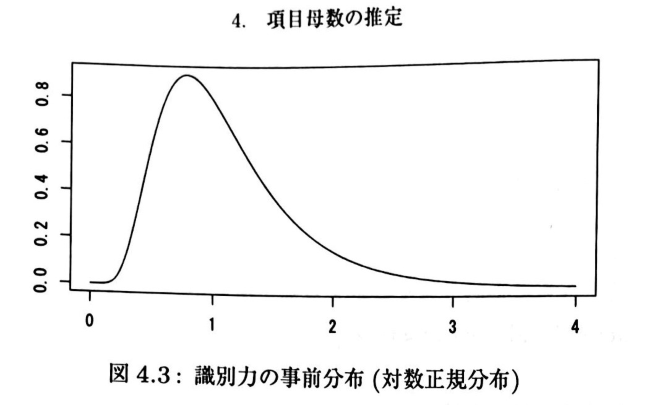
\includegraphics[bb = -500 300 1 1,scale = 0.3]{対数正規分布.png}
\end{figure}
\end{center}
\newpage
\subsubsection{当て推量の事前分布}
当て推量は確率を表現する母数であるため、事前分布も$(0,1)$区間で定義されることが望ましい。このため事前分布はベータ分布が仮定されることが多い。ベータ分布の母数は$\alpha,\beta$であり、ベータ分布の最頻値は、
\begin{align}
  \label{06}
  \displaystyle
  \frac{\alpha - 1}{\alpha + \beta- 2}
  \tag{4.35}
\end{align}
であることが知られている。当て推量の尤もらしい目目安は選択肢数の逆数$c$と考えられる。目安$c$を事前分布の最頻値の一致させるならば、例えば、
\begin{align}
  \label{07}
  \displaystyle
  \alpha = 20 \times c + 1\\
  \beta = 20 \times (1 - c) + 1
  \tag{4.36}
\end{align}
とする。$5$肢選択ならば$c = 0.2$とし$\alpha = 5,\beta = 17$のベータ分布を考える。
\begin{center}
  \begin{figure}[H]
    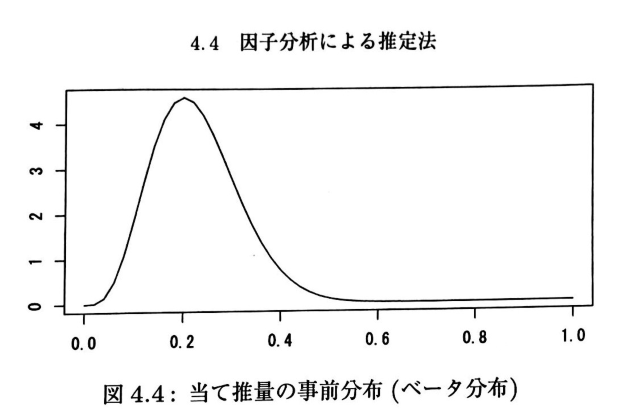
\includegraphics[bb = -500 300 1 1,scale = 0.3]{ベータ分布.png}
  \end{figure}
  \end{center}
\vspace{2cm}
上記の図を見てみると、分布の最頻値が$0.2$であることが確認できる。





\end{document}
